\chapter{Experiments: Regular Tilings}

% (TODO): Overall: standard deviations.

% (TODO): Remember to always specify specifics of experiment setups for all
% experiments

\textcolor{red}{
  \textbf{Methodology:} We look at the three most common types of tilings by
regular polygons: regular tilings. Grünbaum and Shephard (section 1.3) about
tilings, talks about regularity. ``Edge-to-edge'' tiling by congruent regular
polygons. The three regular tesselations, or Euclidean tilings, are square,
triangular, and hexagonal.
}

\textcolor{red}{
  There also exists semiregular, often called uniform, tilings, where there are
two or more faces. There are also more complex schemes, but we are interested in
tilings that are lattice-like. The different types of Bravais lattices for 2
dimensions were all investigated, but using just regular tilings was found to be
sufficient. We are not necessarily interesting in comparing lattice structures
directly, but rather in the applicability of such structures in general.
}

\textcolor{blue}{
  ``Lattice networks/models are common in computational physics, condensed
matter physics and beyond, modelling physical interactions, phase transitions
and structure [15]. Examples include: discrete lattices like the Ising model
with variables representing magnetic dipole moments of atomic spins, and the
Gray- Scott reaction-diffusion model to simulate chemical systems [22]. Also,
physical substrates often have a regular grid of connections. Lattice networks
are therefore more realistic representations of many physical systems that would
be considered for reservoir computing.'', Role of Structure and Complexity, Dale
et al.
}

% (TODO): t!
\begin{figure*}[t]
  \centering
  \begin{subfigure}{.32\textwidth}
    \centering
    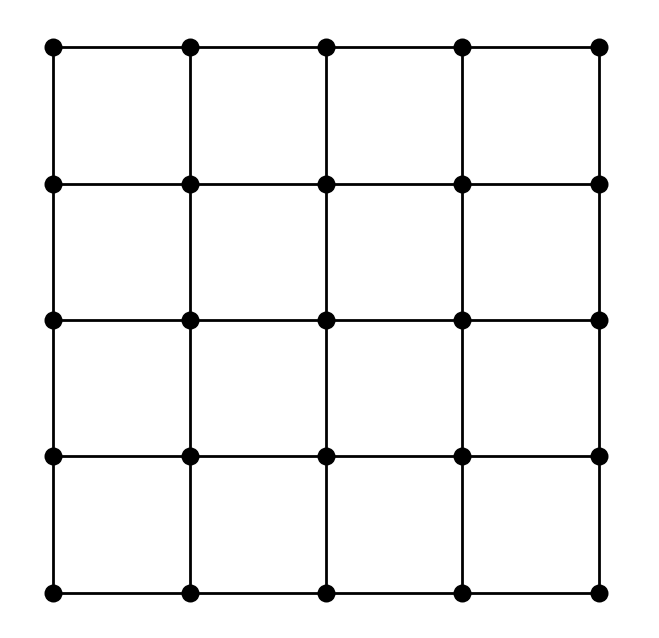
\includegraphics[width=1.0\linewidth]{figures/square.png}
    \label{fig:rt-square}
  \end{subfigure}
  \begin{subfigure}{.32\textwidth}
    \centering
    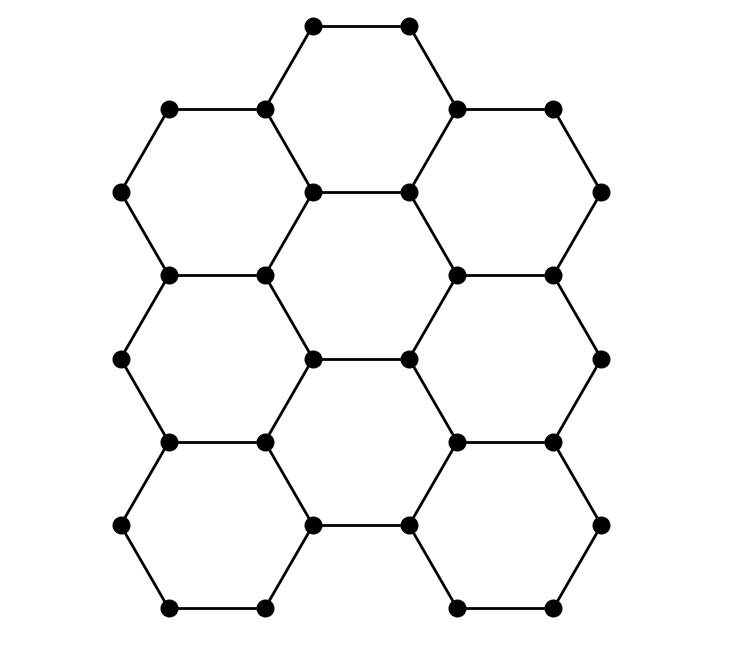
\includegraphics[width=1.0\linewidth]{figures/hex.png}
    \label{fig:rt-hex}
  \end{subfigure}
  \begin{subfigure}{.32\textwidth}
    \centering
    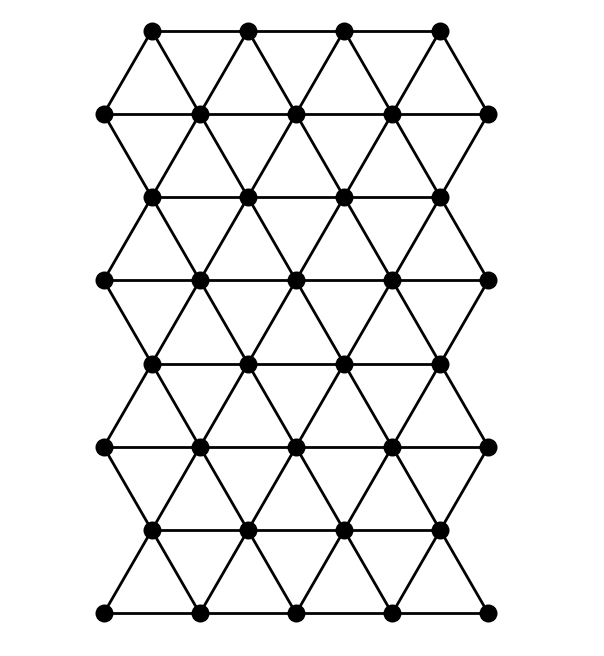
\includegraphics[width=1.0\linewidth]{figures/triangular.png}
    \label{fig:rt-tri}
  \end{subfigure}
  \caption{
    Regular tilings investigated for their quality as reservoir
topologies. Investigated topologies include square (a), hexagonal (b), and
triangular (c) regular tilings.
  }
  \label{fig:regular-tilings}
\end{figure*}

\section{Methodology}

% (TODO): Chapter reference.
\textcolor{red}{
  \textbf{Methodology:} We use the same base as provided by the chapter on
methodology, but replace the weight matrix of the reservoir, i.e. its innards,
with that of the lattice structures we generate. This provides connectivity
within the reservoir of regular, spatially constrained nature. Everything else
should be the same.
}

\section{Reservoir Quality of Regular Tilings}

\subsection{Synopsis}

\subsection{Results and Discussion}

% (TODO): t!
\begin{figure}[t]
  \centering
  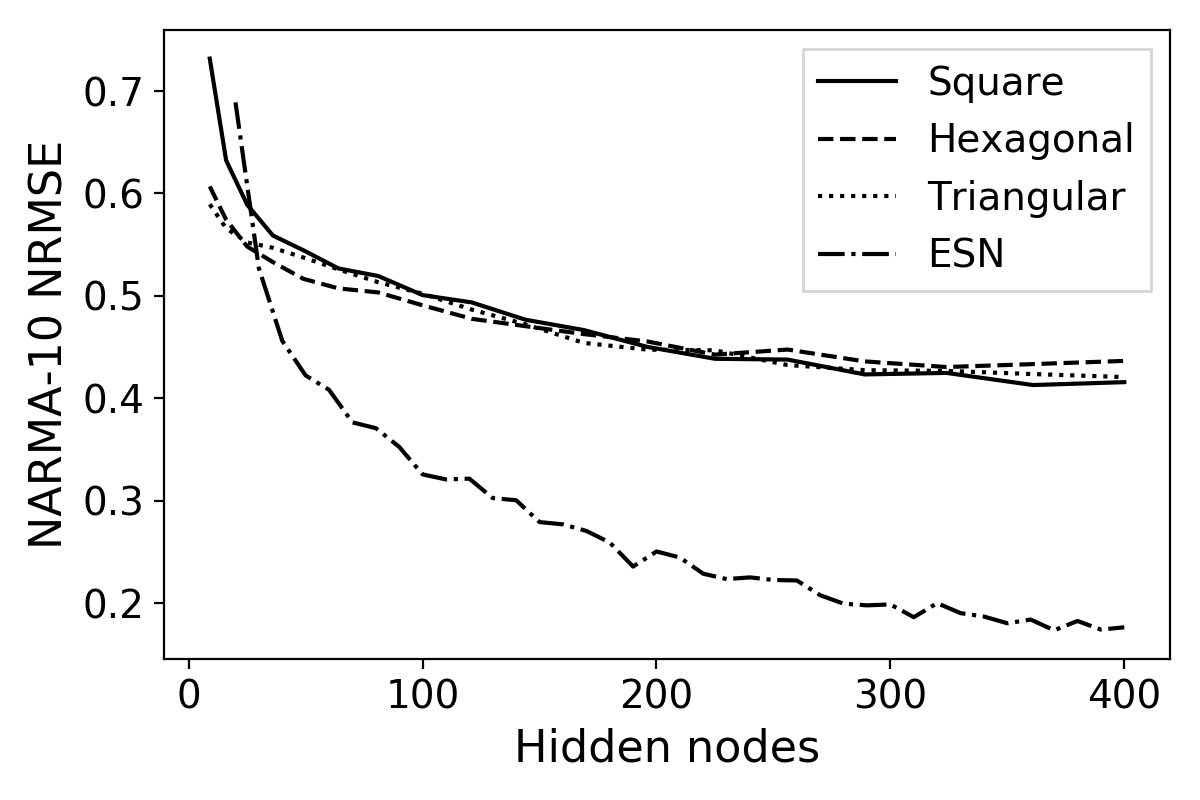
\includegraphics[width=3.5in]{figures/regular-tilings-performance.png}
  \caption{
    Performance of square, hexagonal, and triangular regular tilings as
reservoir topologies without other modifications to the echo state network
methodology.
  }
  \label{fig:rt-performance}
\end{figure}

\textcolor{red}{
  Again, we see that restricting topologies with no other changes will result in
a performance penalty, seen in Figure \ref{fig:rt-performance}.
}

% (TODO): t!
\begin{figure*}[t]
  \centering
  \begin{subfigure}{.32\textwidth}
    \centering
    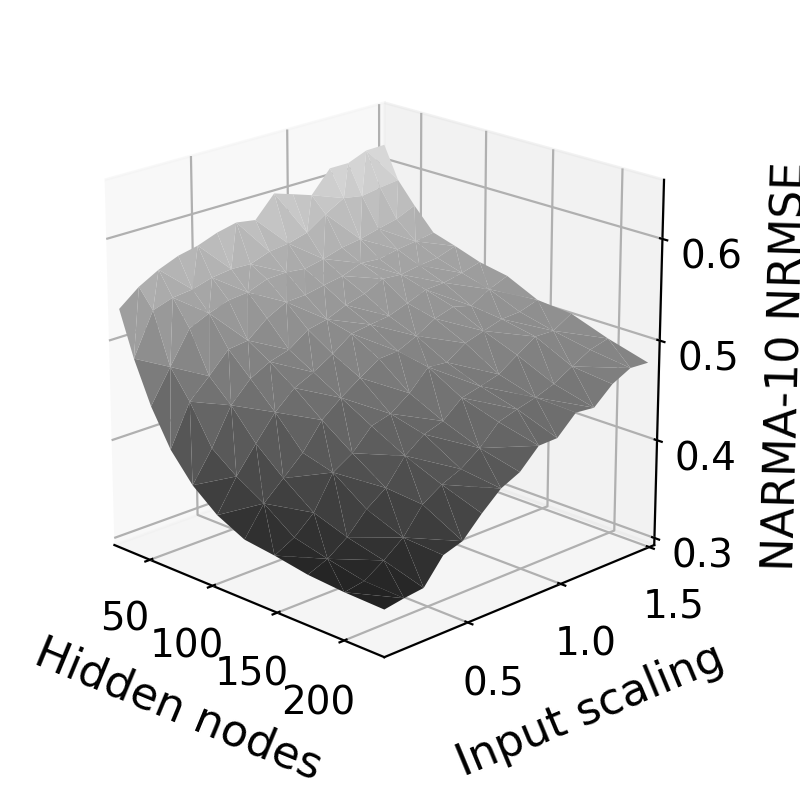
\includegraphics[width=1.0\linewidth]{figures/regular-tilings-performance-is-sq.png}
    \caption{}
    \label{fig:rt-is-square}
  \end{subfigure}
  \begin{subfigure}{.32\textwidth}
    \centering
    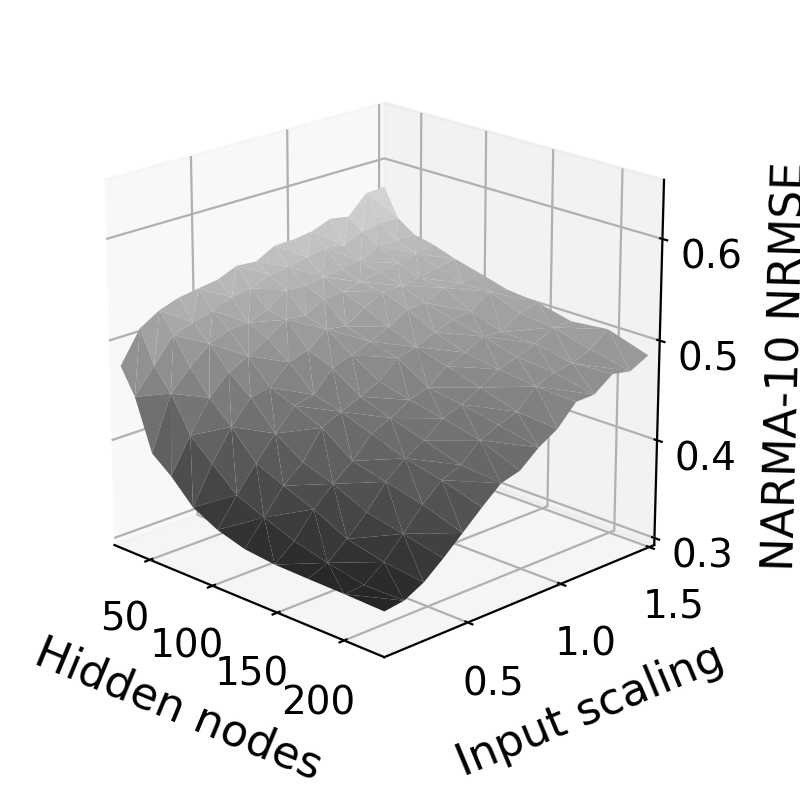
\includegraphics[width=1.0\linewidth]{figures/regular-tilings-performance-is-hex.png}
    \caption{}
    \label{fig:rt-is-hex}
  \end{subfigure}
  \begin{subfigure}{.32\textwidth}
    \centering
    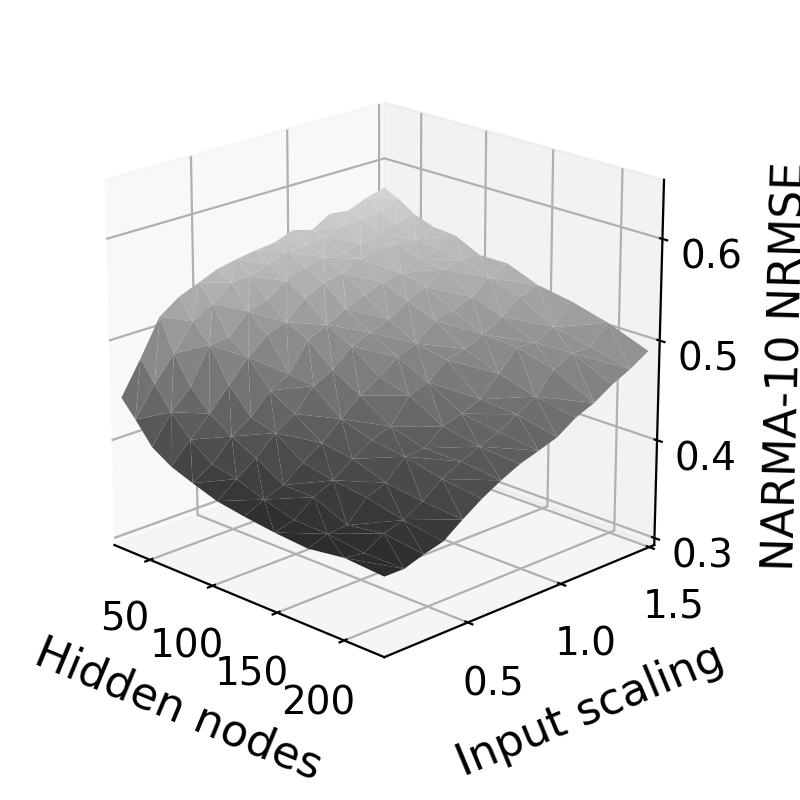
\includegraphics[width=1.0\linewidth]{figures/regular-tilings-performance-is-tri.png}
    \caption{}
    \label{fi:rt-is-tri}
  \end{subfigure}
  \caption{
    Regular tilings investigated for their quality as reservoir topologies, here
as a function of reservoir size and input scaling. Investigated topologies
include square (a), hexagonal (b), and triangular (c) regular tilings.
  }
  \label{fig:rt-performance-is}
\end{figure*}

% (TODO): ref.
\textcolor{red}{
  Further, we investigate the impact of input scaling using what we found in
Chapter ?, as input plays a critical role in input retention. Here, the question
is perhaps not ``exactly how good can we make the topologies with input
scaling'', but we are instead interested in the fact that it does matter at all,
as we can use this in further experiments. We see in Figure
\ref{fig:rt-performance-is} that lowering the input scaling again improves
performance significantly, perhaps again due to issues with memory capacities.
}

\section{Regular Tilings with Directed Edges}

\subsection{Synopsis}

% (TODO): ref.
\textcolor{red}{
Using knowledge obtained in Chapter ?, we modify the resulting networks to have
directed edges, and scale the input magnitude to find a suitable one.
}

\subsection{Results and Discussion}

% (TODO): t!
\begin{figure*}[t]
  \centering
  \begin{subfigure}{.40\textwidth}
    \centering
    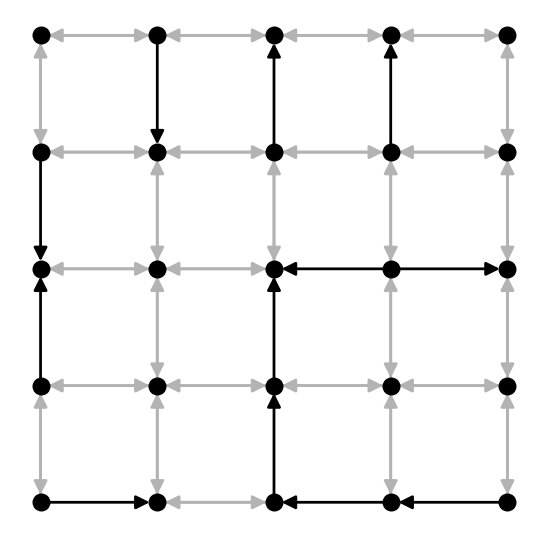
\includegraphics[width=1.0\linewidth]{figures/dir_lattice_025.png}
    \caption{}
    \label{fig:dir-lattice-a}
  \end{subfigure}
  \hspace{25pt}
  \begin{subfigure}{.40\textwidth}
    \centering
    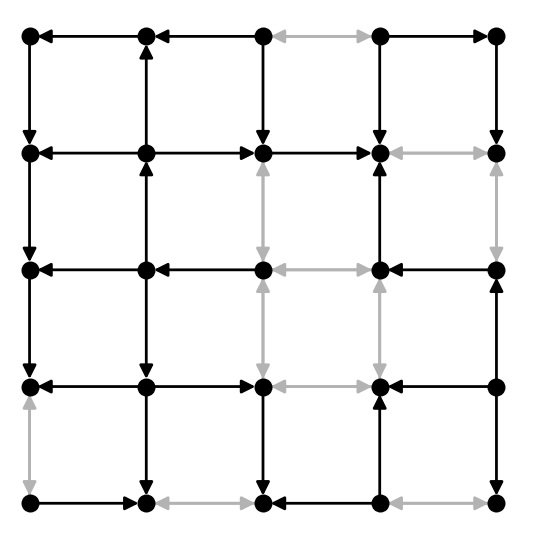
\includegraphics[width=1.0\linewidth]{figures/dir_lattice_075.png}
    \caption{}
    \label{fig:dir-lattice-b}
  \end{subfigure}
  \caption{
    Example square grids where 25\% (a) and 75\% (b) of the undirected edges are
made directed instead.
  }
  \label{fig:dir-lattice}
\end{figure*}

% (TODO): t!
\begin{figure*}[t]
  \centering
  \begin{subfigure}{.32\textwidth}
    \centering
    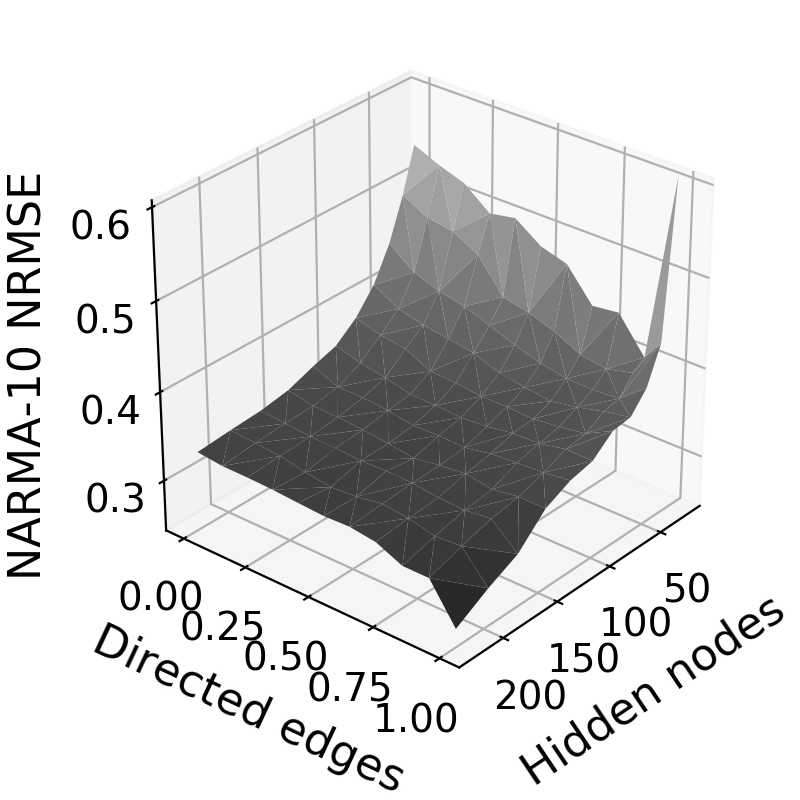
\includegraphics[width=1.0\linewidth]{figures/rt-dir-perf-sq.png}
    \caption{}
    \label{fig:rt-dir-perf-trisurf-sq}
  \end{subfigure}
  \begin{subfigure}{.32\textwidth}
    \centering
    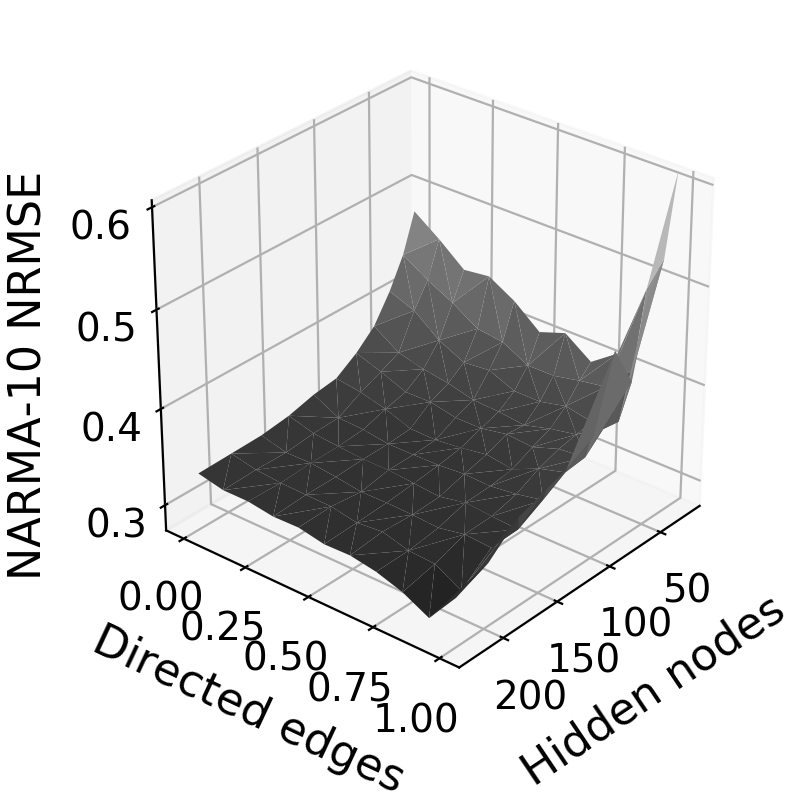
\includegraphics[width=1.0\linewidth]{figures/rt-dir-perf-hex.png}
    \caption{}
    \label{fig:rt-dir-perf-trisurf-hex}
  \end{subfigure}
  \begin{subfigure}{.32\textwidth}
    \centering
    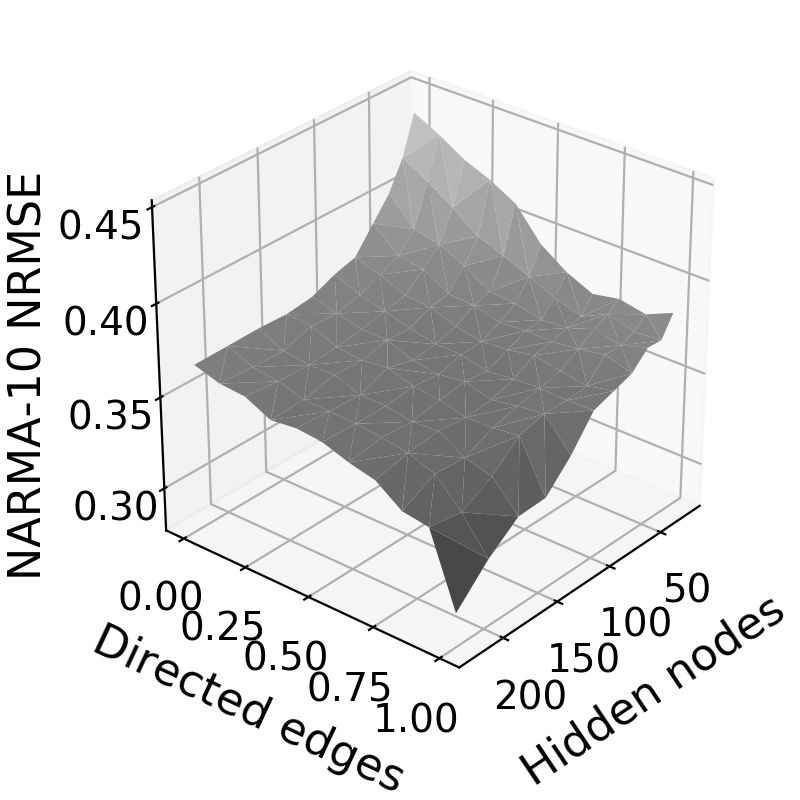
\includegraphics[width=1.0\linewidth]{figures/rt-dir-perf-tri.png}
    \caption{}
    \label{fig:rt-dir-perf-trisurf-tri}
  \end{subfigure}
  \caption{
    \textcolor{red}{No caption yet.}
  }
  \label{fig:rt-dir-perf-trisurf}

  \centering
  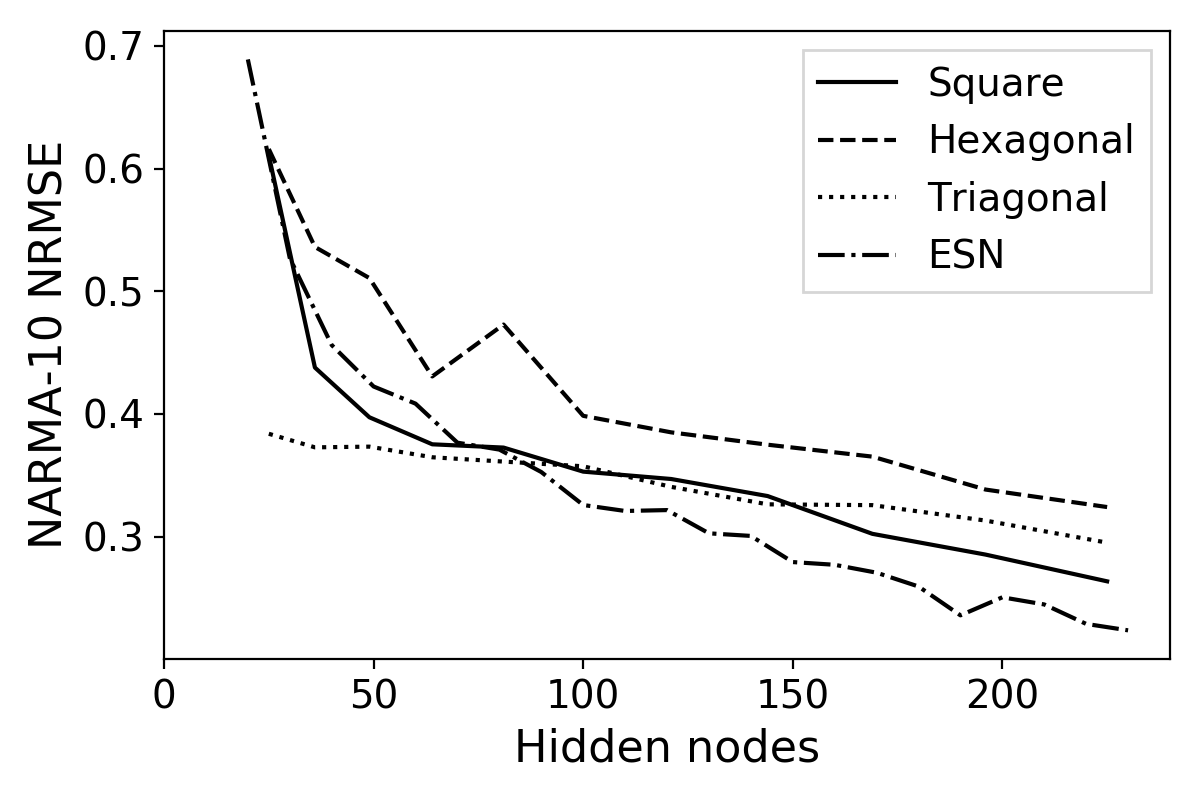
\includegraphics[width=3.5in]{figures/rt-dir-perf.png}
  \caption{\textcolor{red}{No caption yet here.}}
  \label{fig:rt-dir-perf}
\end{figure*}

\textcolor{red}{
  We see that directed edges make the grids perform quite close to ESNs on the
NARMA-10 dataset. We choose the square lattice to move further, as they are all
quite similar, but the square one seems most stable and performs very well.
}

\begin{figure}
  \centering
  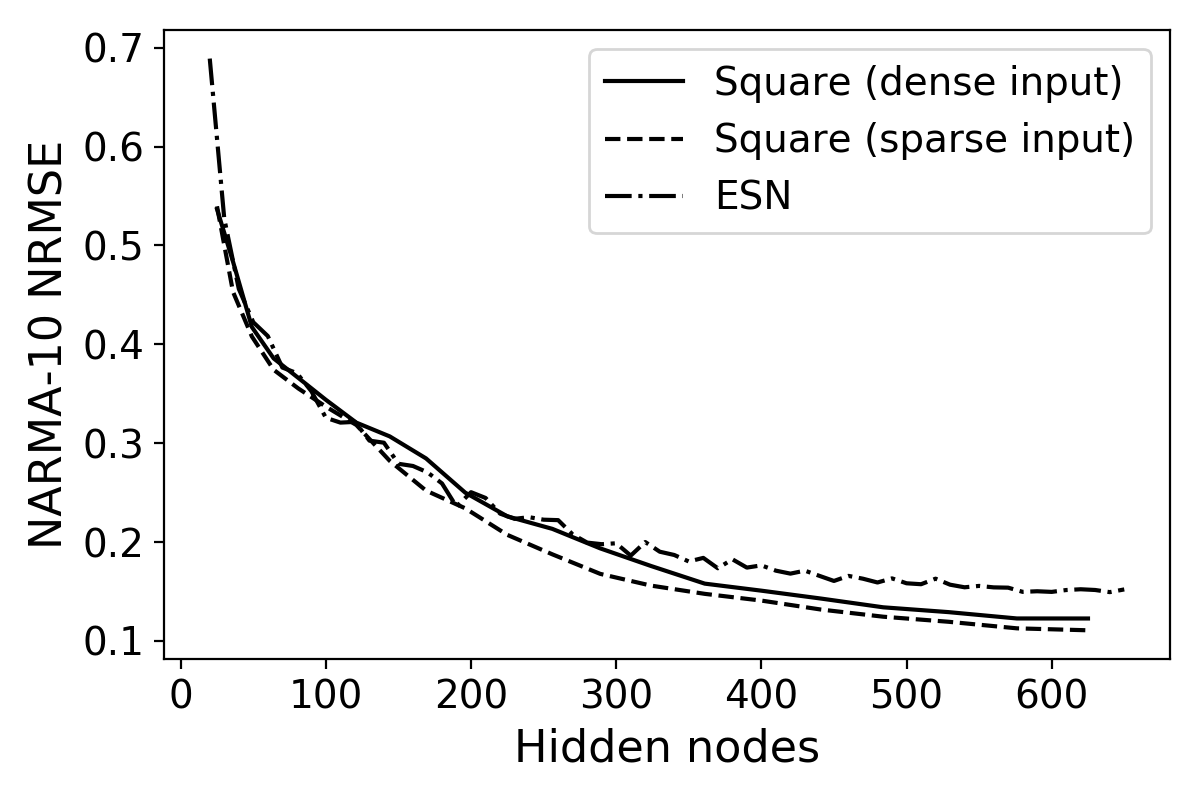
\includegraphics[width=3.5in]{figures/rt-performance-big.png}
  \caption{\textcolor{red}{No caption here yet.}}
  \label{fig:rt-performance-big}
\end{figure}

\textcolor{red}{
  When we introduce a global input scheme, the square grids get even
better. This is crazy. The square grids do not plateau nearly as much as the
ESNs. In fact they get much better. We also add sparse input matrices, which
means only 50\% of the hidden nodes see the input.
}

% (TODO): t!
\begin{table}[t]
  \centering
  \begin{center}
    \caption{
      \textcolor{red}{
        Simple weighting scheme of square grids. Displayed values are given as
an average across 10 experiment runs (std. dev.). Reservoir connectivity density
in ESNs is 10\%.
      }
    }
    \label{tab:sq-global-input}
    \begin{tabular}{c c c c c}
      \hline
      \thead{Reservoir type} & \thead{Hidden \\ nodes} & \thead{Unique \\ input weights} & \thead{Unique \\ reservoir weights} & \thead{NARMA-10 \\ NRMSE} \\
      \hline
      \rule{0pt}{2.5ex}Square grid & 100 & 1 & 1 & 0.346 (0.019) \\
      Square grid & 225 & 1 & 1 & 0.245 (0.022) \\
      Square grid & 400 & 1 & 1 & 0.168 (0.009) \\
      \rule{0pt}{3ex}ESN & 100 & 100 & 997 (26) & 0.388 (0.019) \\
      ESN & 225 & 225 & 5098 (74) & 0.282 (0.019) \\
      ESN & 400 & 400 & 16070 (113) & 0.215 (0.021)\rule[-1ex]{0pt}{0pt} \\
      \hline
    \end{tabular}
  \end{center}
\end{table}

% (TODO): t!
\begin{figure*}[t]
  \centering
  \begin{subfigure}{.49\textwidth}
    \centering
    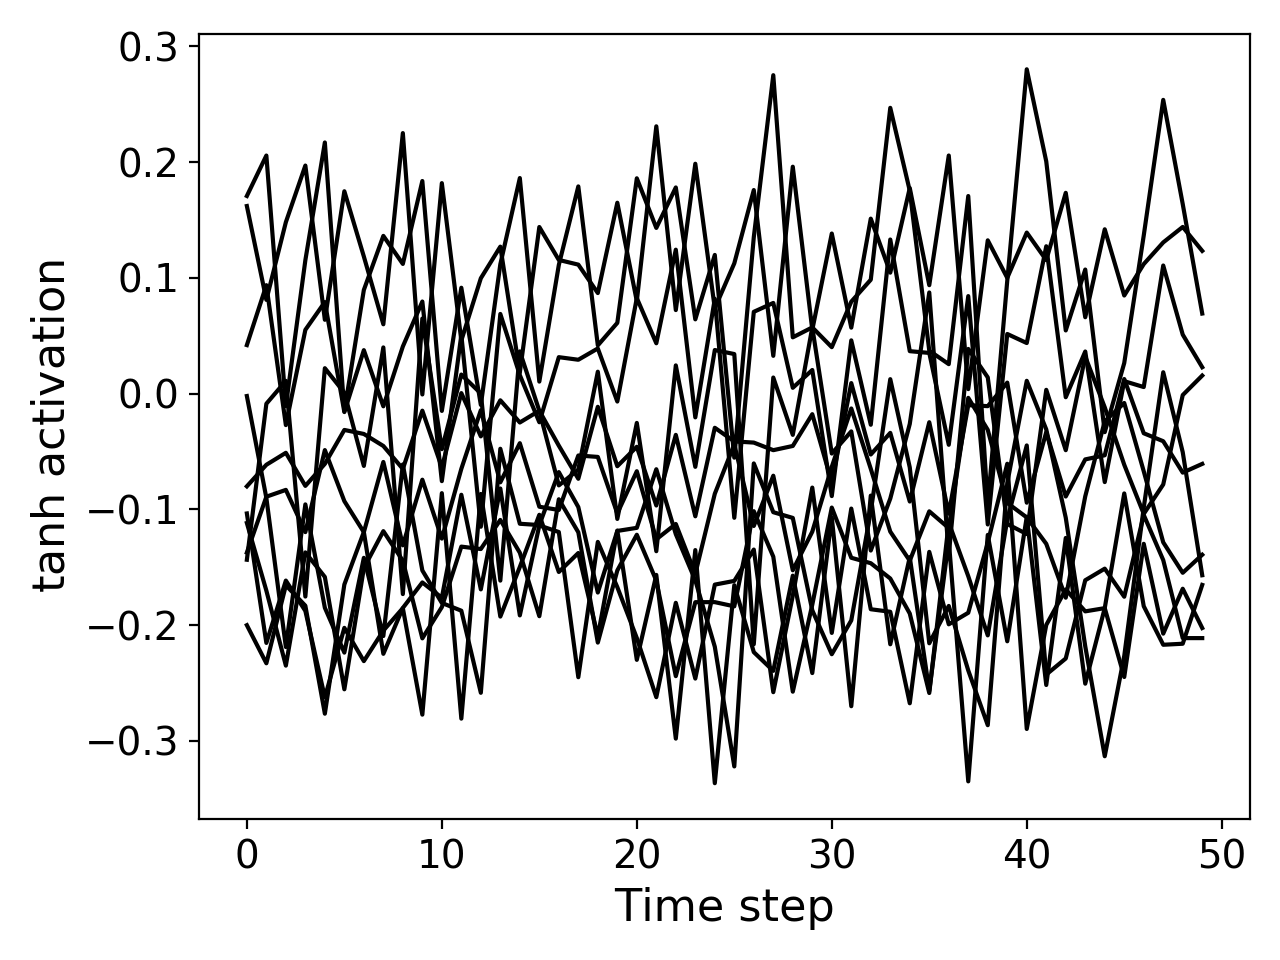
\includegraphics[width=1.0\linewidth]{figures/esn-activations.png}
    \caption{}
    \label{fig:activations-a}
  \end{subfigure}
  \begin{subfigure}{.49\textwidth}
    \centering
    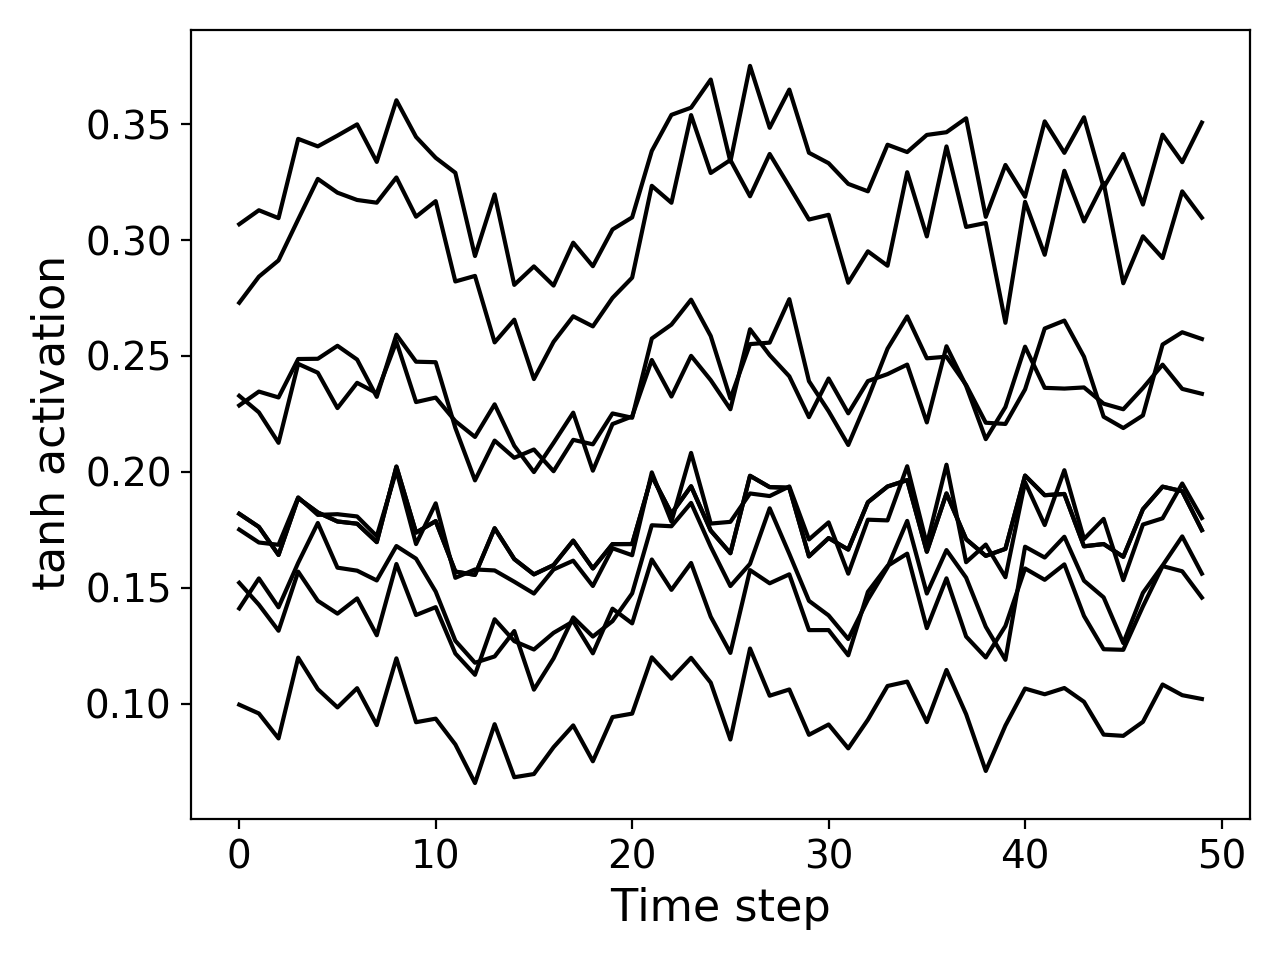
\includegraphics[width=1.0\linewidth]{figures/sq-activations.png}
    \caption{}
    \label{fig:activations-b}
  \end{subfigure}
  \caption{
    \textcolor{red}{
      This is only 10 of the nodes to give an example without cluttering too
much. Square grid has only positive activations, and the input is clearly
visible, while the ESN is sporadic, random.
    }
  }
  \label{fig:activations}
\end{figure*}

\textcolor{red}{
  After looking at the activations here, all positive, one may consider other
sigmoid functions of course, but experiments showed $tanh$ to work just fine.
}

\textcolor{red}{
  We should maybe also compare MC and KQ/G to that of ESNs, as independent
metrics. We see that the square grids have a much lower kernel quality,
i.e. less dynamics, which may impact performance. However, some studies with
Mackey-Glass indicate that it will also work for that. So there is this
trade-off to make the square grid work, in that the dynamics are lessened for
memory, but it \textit{works}, which is the key.
}

\textcolor{red}{
  Should we include experiments with harder NARMA? I think there is already
quite a lot of information, so this might not really be necessary.
}

\section{Shrinking and Growing Square Grids}

\subsection{Synopsis}

\subsection{Results and Discussion}

\begin{figure}
  \centering
  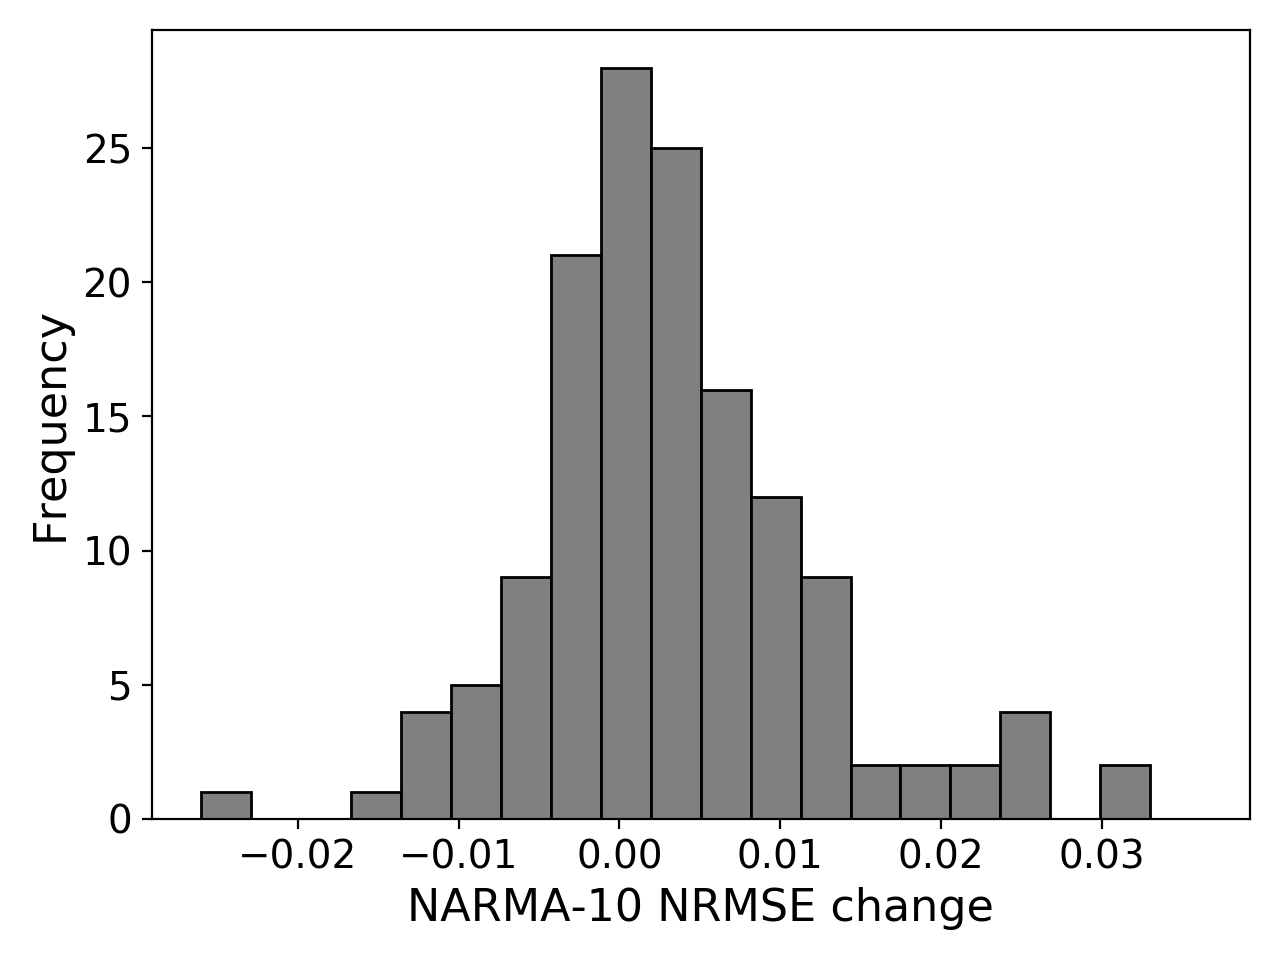
\includegraphics[width=3.5in]{figures/removal-hist.png}
  \caption{
    \textcolor{red}{
      Impact on NARMA-10 NRMSE when removing nodes from a 12x12 square grid
reservoir. No nodes are absolutely essential, while some removals actually
improve overall performance.
    }
  }
  \label{fig:rt-removal-hist}
\end{figure}

\begin{figure}
  \centering
  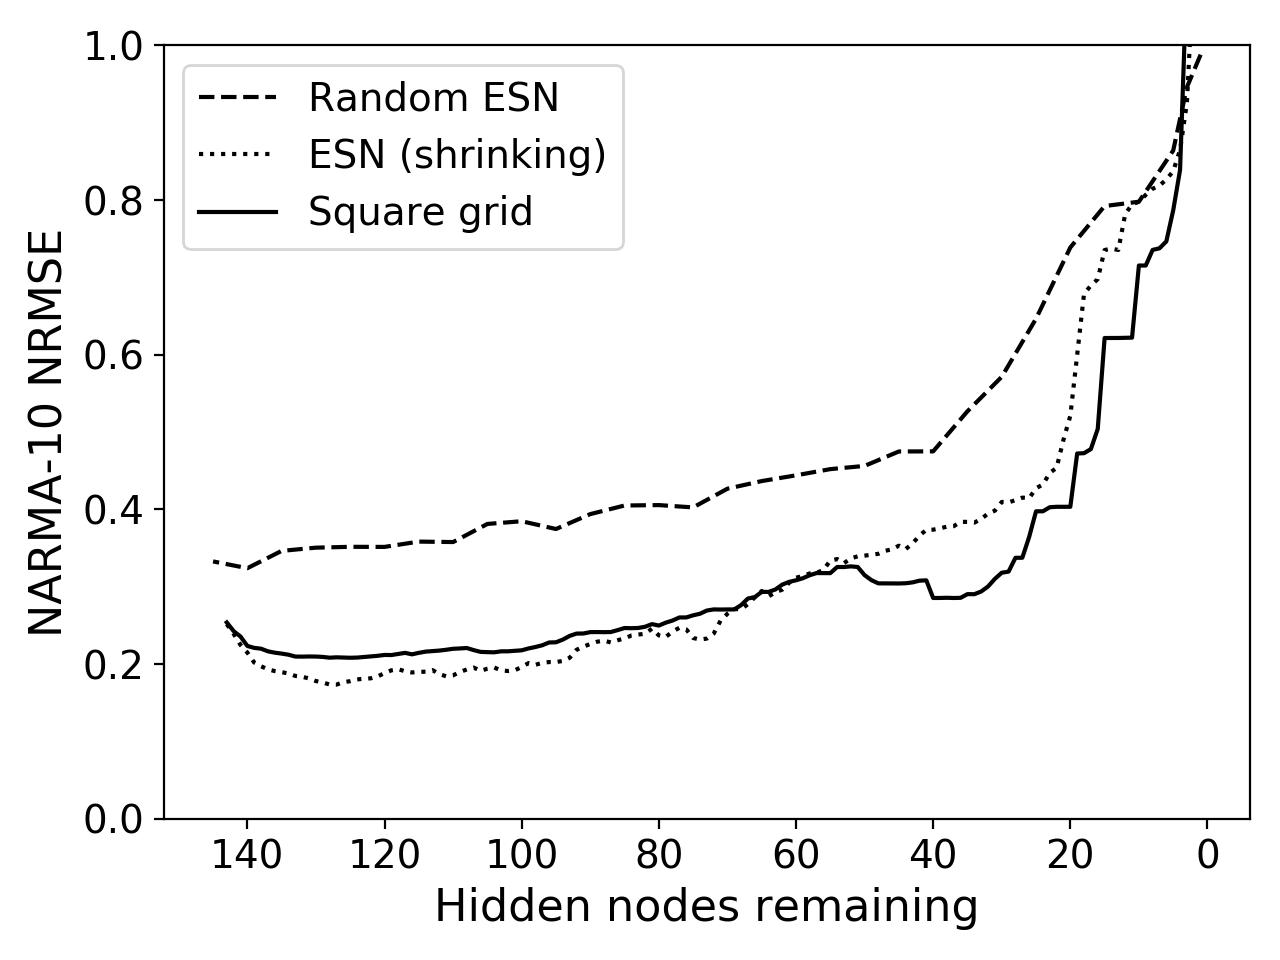
\includegraphics[width=3.5in]{figures/shrink-performance.png}
  \caption{
    \textcolor{red}{
      No caption yet.
    }
  }
  \label{fig:sq-shrink-performance}
\end{figure}

% (TODO): t!
\begin{figure*}[t]
  \centering
  \begin{subfigure}{.40\textwidth}
    \centering
    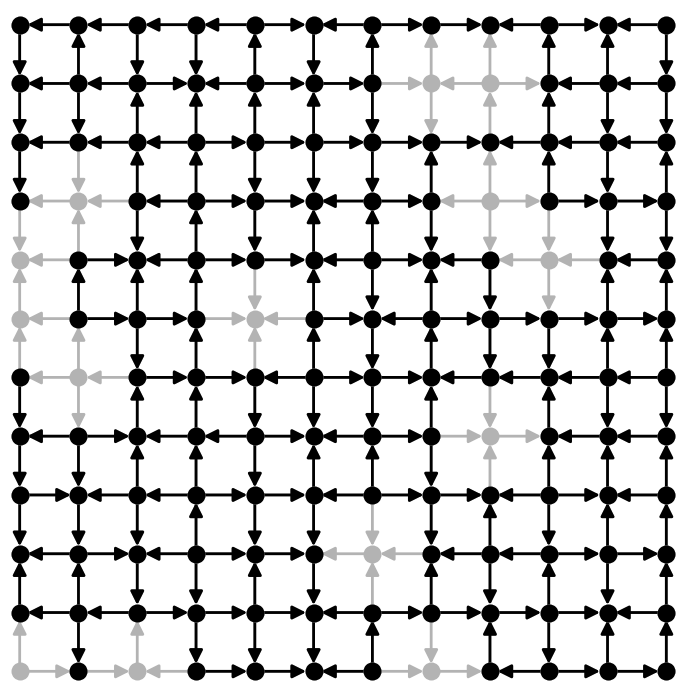
\includegraphics[width=1.0\linewidth]{figures/sq-grid-130.png}
    \caption{}
    \label{fig:sq-grid-130}
  \end{subfigure}
  \begin{subfigure}{.40\textwidth}
    \centering
    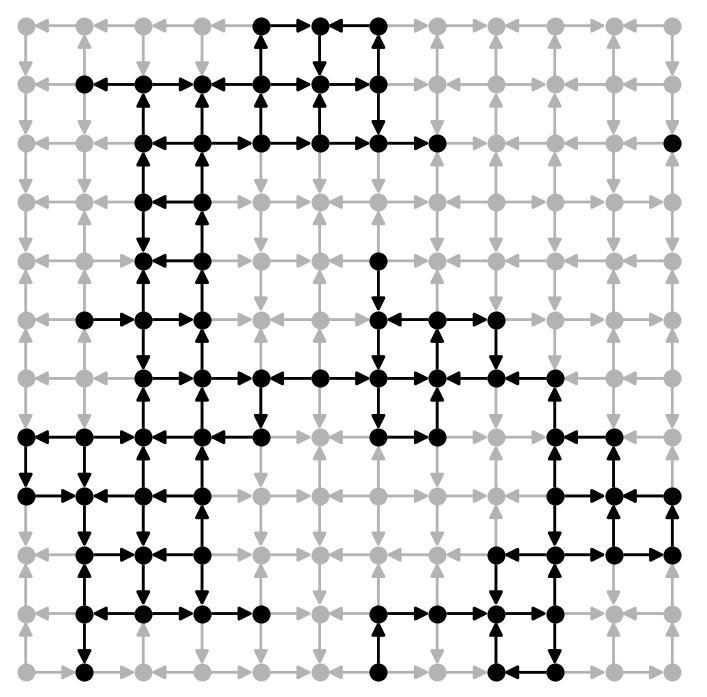
\includegraphics[width=1.0\linewidth]{figures/sq-grid-70.png}
    \caption{}
    \label{fig:sq-grid-70}
  \end{subfigure}
  \vskip\baselineskip

  \begin{subfigure}{.40\textwidth}
    \centering
    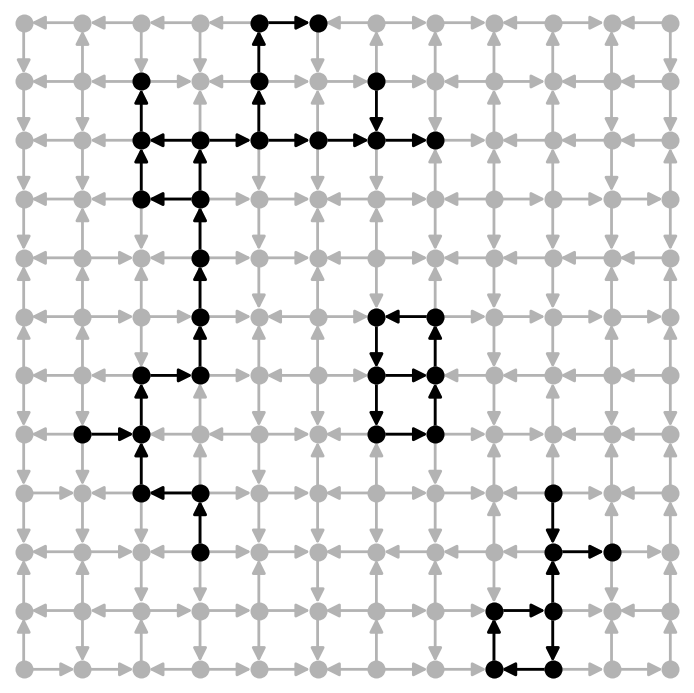
\includegraphics[width=1.0\linewidth]{figures/sq-grid-35.png}
    \caption{}
    \label{fig:sq-grid-35}
  \end{subfigure}
  \begin{subfigure}{.40\textwidth}
    \centering
    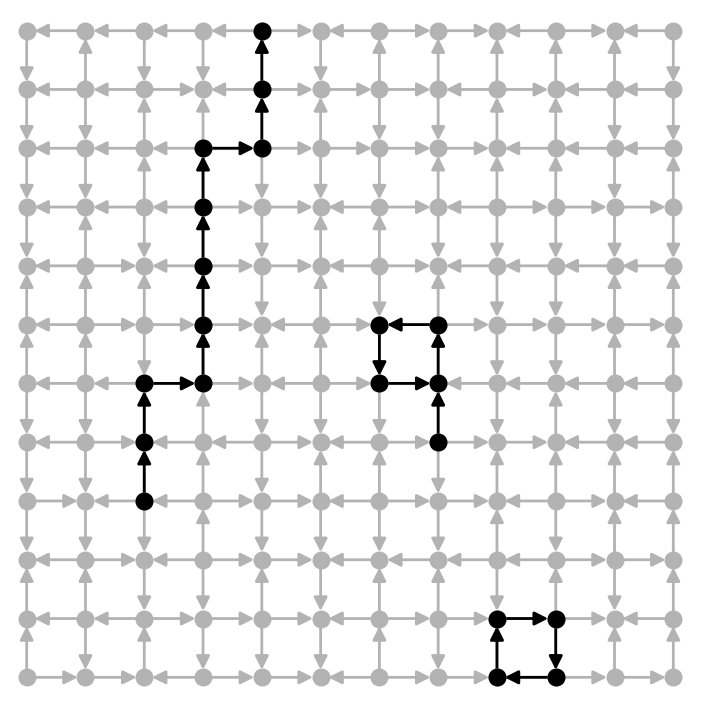
\includegraphics[width=1.0\linewidth]{figures/sq-grid-20.png}
    \caption{\textcolor{red}{Should have NRMSE and nodes left here.}}
    \label{fig:sq-grid-20}
  \end{subfigure}
  \caption{
    \textcolor{red}{
      Progression when incrementally removing nodes from a 12x12 square grid.
    }
  }
  \label{fig:sq-grid}
\end{figure*}

\textcolor{red}{
  Add the example when we have removed nodes from ESN? The one that is just
impossible to make sense of. This is common knowledge however, we could probably
just mention that.
}

\textcolor{red}{
  We need to stress that this is just one example, there is no variance here,
which is a bit of a weakness in the argument.
}

\begin{figure}
  \centering
  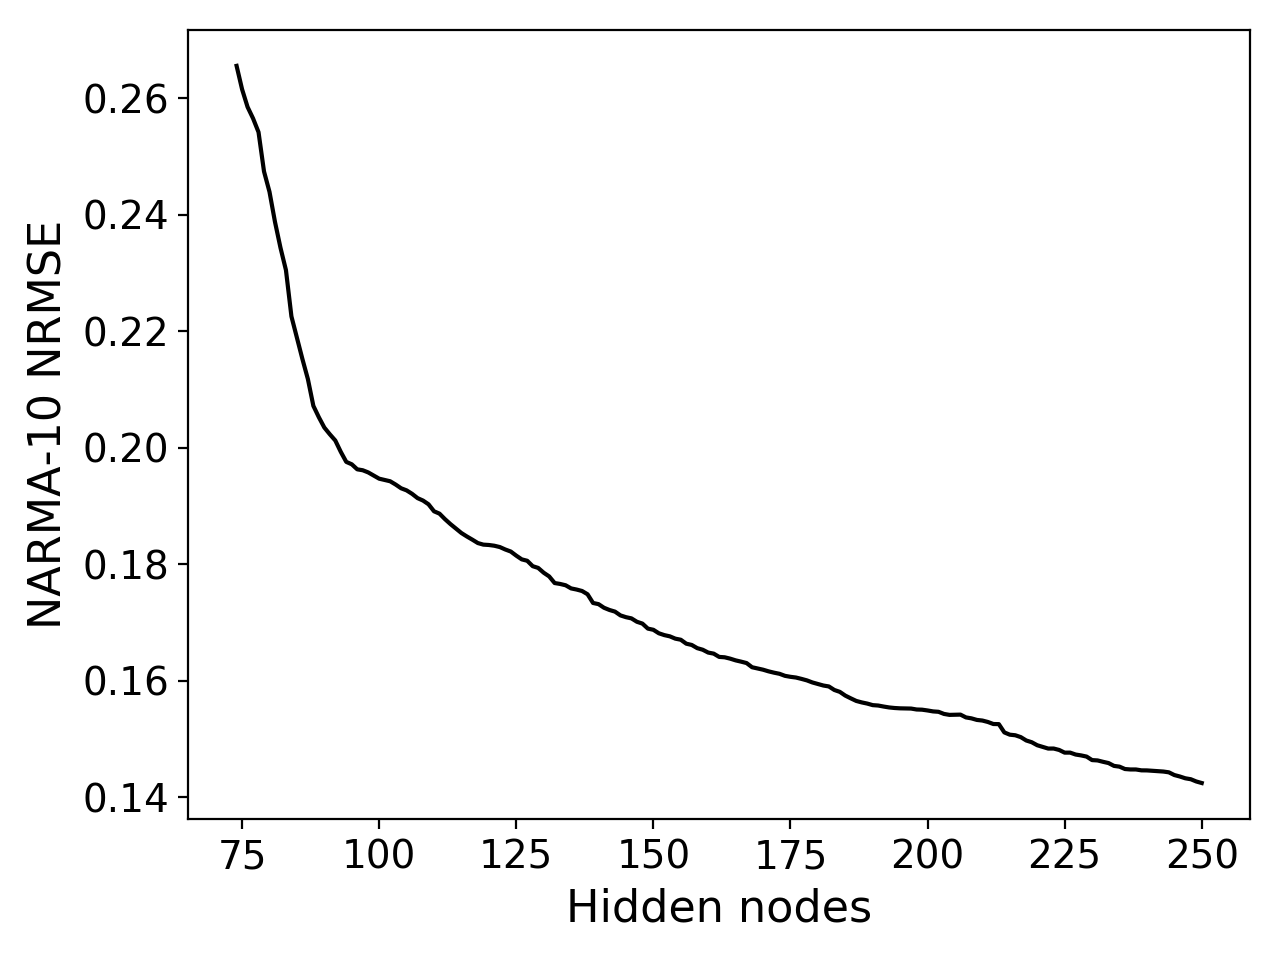
\includegraphics[width=3.5in]{figures/grow-performance.png}
  \caption{
    \textcolor{red}{
      No caption yet.
    }
  }
  \label{fig:sq-grow-performance}
\end{figure}

% (TODO): t!
\begin{figure*}[t]
  \centering
  \begin{subfigure}{1.0\textwidth}
    \centering
    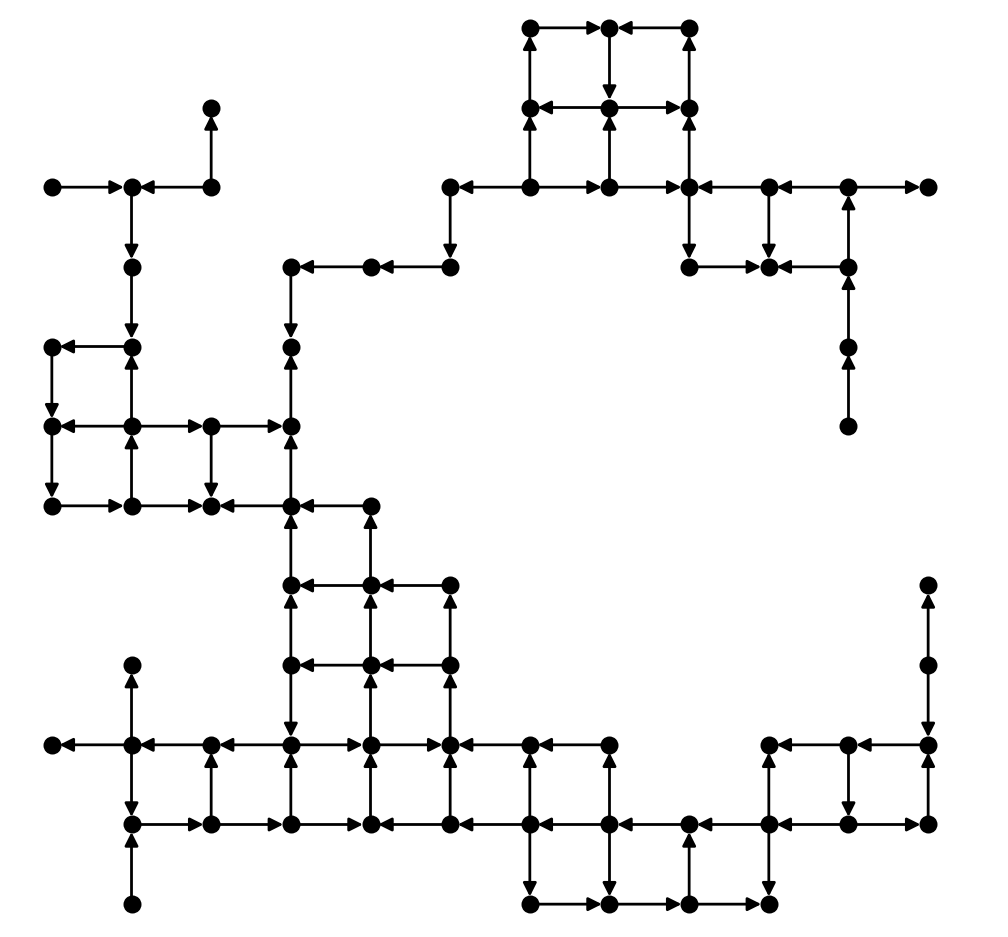
\includegraphics[width=0.5\linewidth]{figures/sq-grid-grow-74.png}
    \caption{}
    \label{fig:sq-grid-grow-74}
  \end{subfigure}
  \begin{subfigure}{.49\textwidth}
    \centering
    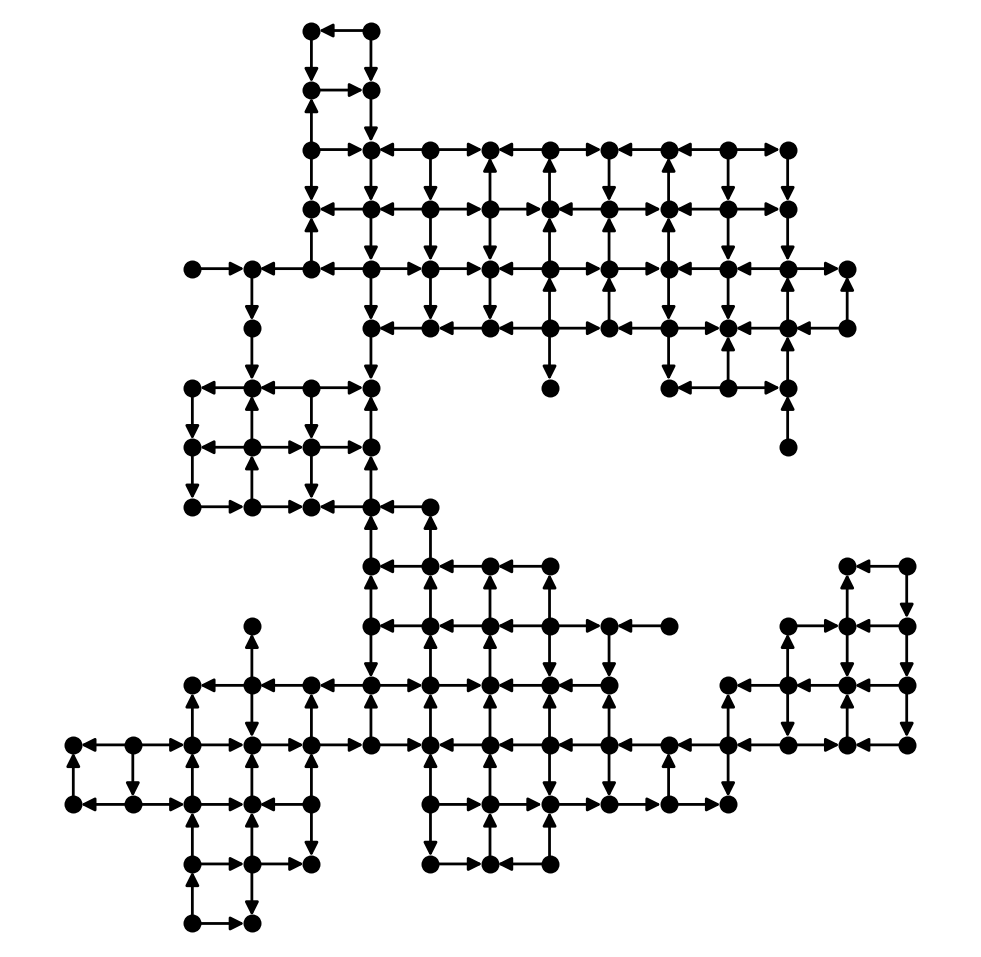
\includegraphics[width=1.0\linewidth]{figures/sq-grid-grow-124.png}
    \caption{}
    \label{fig:sq-grid-grow-124}
  \end{subfigure}
  \begin{subfigure}{.49\textwidth}
    \centering
    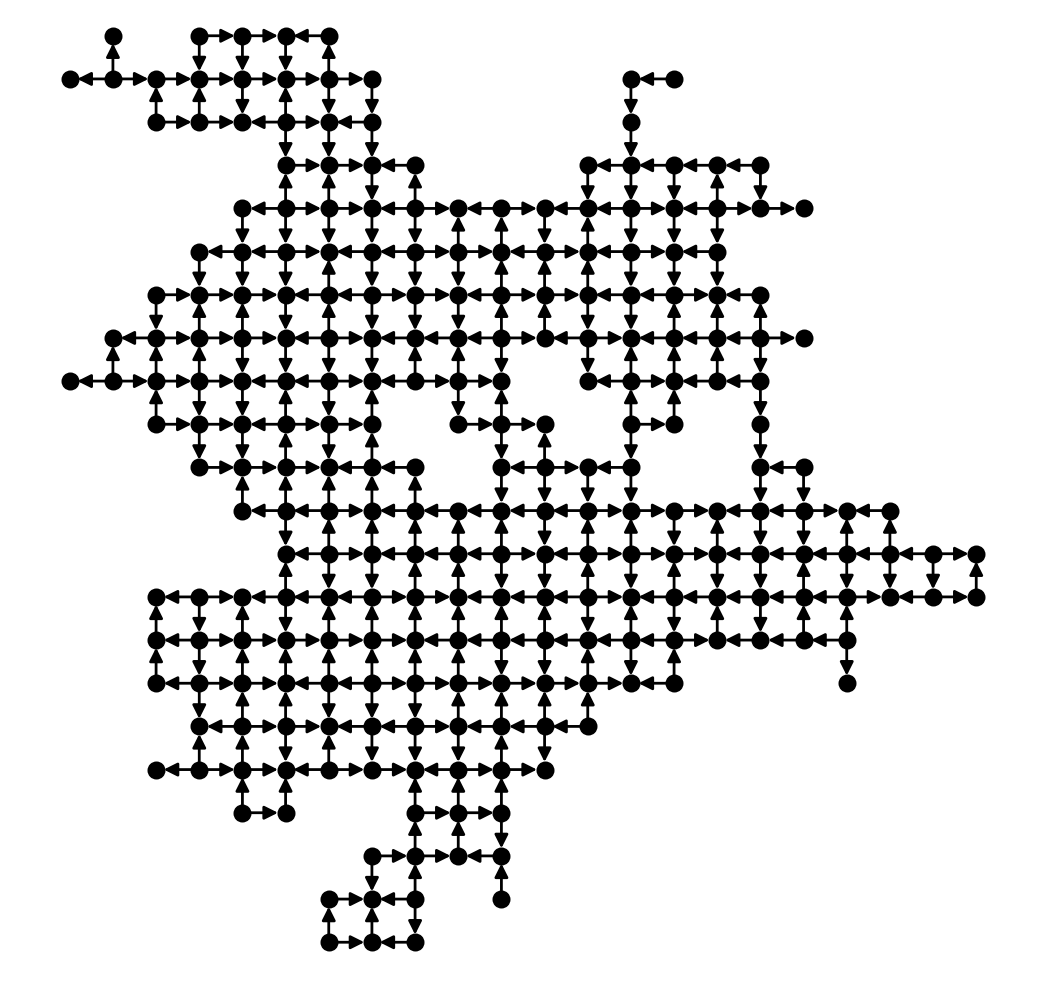
\includegraphics[width=1.0\linewidth]{figures/sq-grid-grow-250.png}
    \caption{\textcolor{red}{Should have captions for NRMSE and size.}}
    \label{fig:sq-grid-grow-250}
  \end{subfigure}
  \caption{
    \textcolor{red}{
      Caption. We see the initial reservoir from where we start growing in (a),
and progress in (b, c).
    }
  }
  \label{fig:sq-grid-grow}
\end{figure*}

\textcolor{red}{
  We repeat the experiment, but this time \textit{adding} nodes along the
frontier, as we can exhaust every possibility for every iteration without that
much trouble. Harder to see what is happening now.
}

\section{Restoring Bidirectional Edges}

\subsection{Synopsis}

\subsection{Results and Discussion}

\begin{figure}
  \centering
  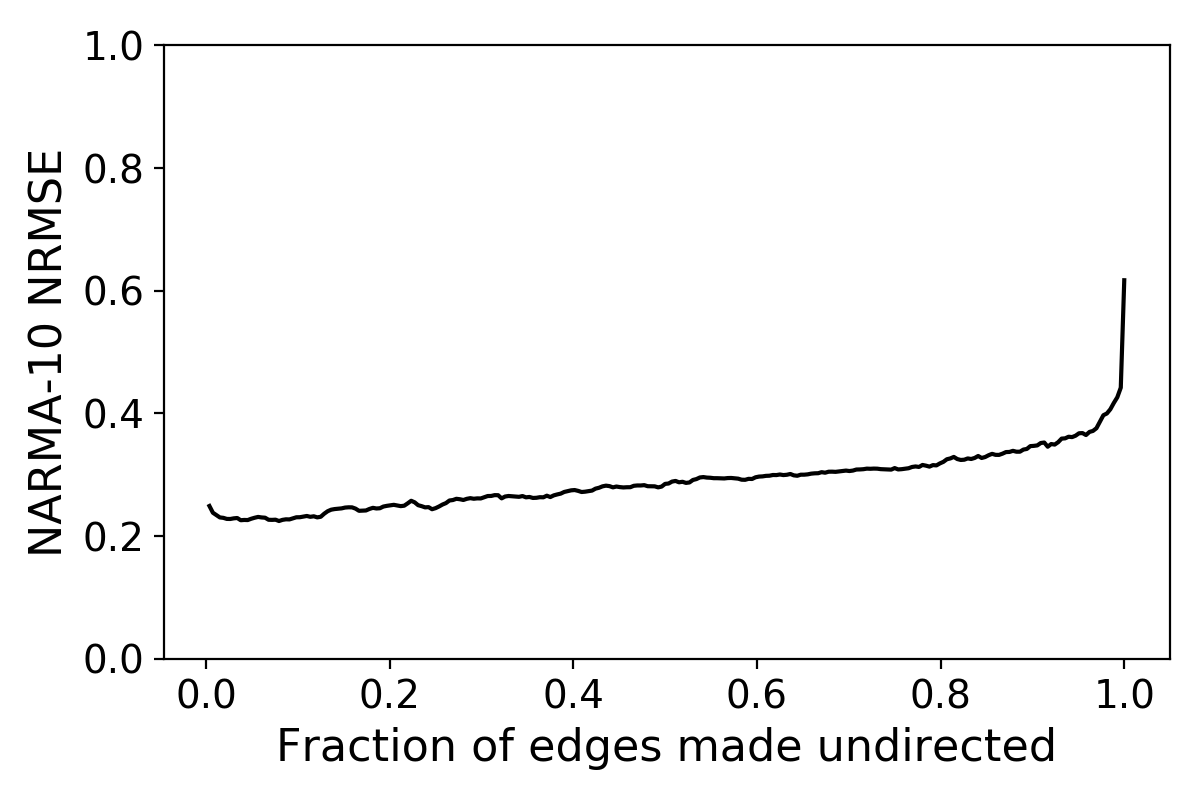
\includegraphics[width=3.5in]{figures/undir-performance.png}
  \caption{
    \textcolor{red}{
      No caption yet. 12x12 square grid.
    }
  }
  \label{fig:undirection-performance}
\end{figure}

\textcolor{red}{
  Imagine something similar to that of Figure \ref{fig:dir-lattice}, where now
only a fraction of the edges are directed again. However, we cannot directly
compare this to that of a cross section of that plot, as we have changed our
input scheme to be global, instead of the uniform distribution that was used
before.
}

\section{Conclusion}


%%% Local Variables:
%%% mode: latex
%%% TeX-master: "../thesis"
%%% End:
